\documentclass[serif,professionalfonts,svgnames]{beamer}
\usepackage{pxfonts}
\usepackage{eulervm}

\usepackage{graphicx}
\usepackage{booktabs}
\usepackage{natbib}
\usepackage{tikz}
\usepackage{pdfsync}
\usepackage{listings}
\usepackage{fancyvrb}

\usetikzlibrary{arrows,shapes,fadings}
\graphicspath{{Images/}}

\newcommand{\admixture}{\textsc{ADMIXTURE}}
\renewcommand{\structure}{\textsc{STRUCTURE}}
\newcommand{\frappe}{\textsc{FRAPPE}}
\newcommand{\eigenstrat}{\textsc{EIGENSTRAT}}
\newcommand{\mendel}{\textsc{MENDEL}}

\def\E{\mathop{\rm E\,\!}\nolimits}
\def\Var{\mathop{\rm Var}\nolimits}
\def\Pr{\mathop{\rm Pr\,\!}\nolimits}

\def\muhat{\hat{\mu}}

\title{Genetic Disease Studies in Structured Populations}
\author{David Alexander}
\date{August 18, 2010}

\mode<presentation>
%{ \usetheme{Goettingen} }

% this is needed for bibliographies to work with beamer
\def\newblock{\hskip .11em plus .33em minus .07em}

\begin{document}
\setlength{\parskip}{10pt plus 1pt minus 1pt}

\maketitle

\begin{frame}{What is population structure?}
  People in the United States draw their ancestry from many distinct
  worldwide populations that evolved in partial isolation. This is the
  essence of a \emph{structured} or \emph{stratified} population.
  Furthermore, there are people who have partial ancestry stemming
  from several different ancestral populations (\emph{admixture}).

  What are the implications for genetic epidemiology?  
\end{frame}

\begin{frame}{We need to account for ancestry in genetic disease studies?}
        An light-hearted example from [Lander \& Schork, 2006]:
        
\begin{quote}   
  ... suppose that a would-be geneticist set out to study the ``trait'' of ability to eat with chopsticks in the San Francisco population by performing an association study with the HLA complex. The allele HLA-A1 would turn out to be positively associated with ability to use chopsticks---not because immunological determinants play any role in manual dexterity, but simply because the allele HLA-A1 is more common among Asians than Caucasians.
\end{quote}
\end{frame}


\begin{frame}{Ancestry acts as a hidden confounder}
  \begin{center}
        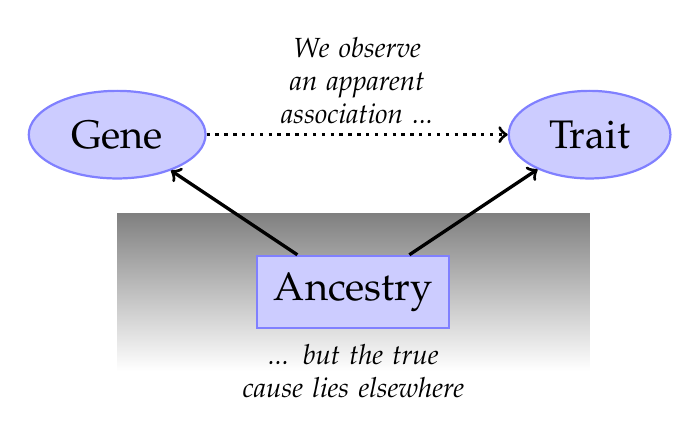
\begin{tikzpicture} 
          [observed/.style={ellipse,draw=blue!50,fill=blue!20,thick,  inner sep=6pt,minimum size=6mm},
          hidden/.style={rectangle,draw=blue!50,fill=blue!20,thick,inner sep=6pt,minimum size=4mm}]
          % \draw[help lines] (-3,-3) grid (3,3);
          \fill [gray,path fading=south] (-3,-3) rectangle (3,-1); 
          \node[observed] (gene)            at (-3,0) {\Large Gene};
          \node[observed] (trait)           at (3, 0) {\Large Trait};
          \node[hidden]   (ancestry)  at (0,-2) {\Large Ancestry};
          \draw[->,very thick,dotted]  (gene) -- (trait) 
          node[above,text width=1in, text centered, midway] 
          {\em We observe an apparent association ...};
          \draw[->,very thick]  (ancestry) -- (trait);
          \draw[->,very thick]  (ancestry) -- (gene);
          \node[text width=2in, text centered] at (0,-3) 
          {\em ... but the true cause lies elsewhere};
        \end{tikzpicture} 
  \end{center}
\end{frame}


\begin{frame}{A simple example of confounding}
\begin{columns}[c]
 \column{2.2in}
 \bigskip
\begin{block}{European sample, $n=120$}
   \small
   \begin{center}
     \colorbox{red!20}{
      \begin{tabular}{lccc}
        & \multicolumn{2}{c}{Disease} &          \\
        \cmidrule{2-3}                             
                   &         +        &               -   \\  \midrule  
        WT         &        60        &              20   \\
        Mutant     &        30        &              10
      \end{tabular}
    }
    $$\widehat{OR} = 1$$
  \end{center}
\end{block}
\vspace{-1cm}
\begin{block}{Amerindian sample, $n=120$}
  \small
  \begin{center}
  \colorbox{blue!20}{
    \begin{tabular}{lccc}
      & \multicolumn{2}{c}{Disease} &          \\
      \cmidrule{2-3}                             
                 &         +        &               -   \\  \midrule  
      WT         &        10        &              30   \\
      Mutant     &        20        &              60
    \end{tabular}
  }
  $$\widehat{OR} = 1$$
  \end{center}
 \end{block}
 \column{2.5in}
 \pause
 \begin{block}{Pooled samples, $n=240$}
   \small
   \begin{center}
     \colorbox{purple!20}{
       \begin{tabular}{lccc}
         & \multicolumn{2}{c}{Disease} &          \\
         \cmidrule{2-3}                             
                    &         +        &               -   \\  \midrule  
         WT         &        70        &              50   \\
         Mutant     &        50        &              70
       \end{tabular}
     }
   \end{center}

   $${\bf \widehat{OR} = 1.96}$$
 \end{block}
\end{columns}
\end{frame}


\begin{frame}
\frametitle{A real world example, and its lessons}
\begin{itemize}
\item{The classic Pima Indian Diabetes study [Knowler, 1988]

\begin{center}
\fbox{
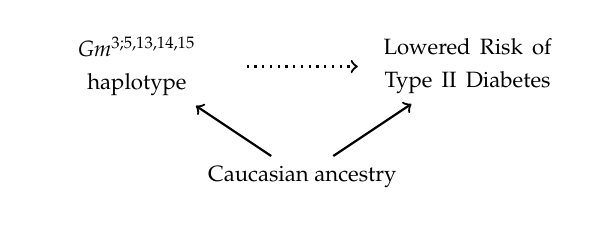
\begin{tikzpicture}[scale=0.7] 
		[observed/.style={},
		 hidden/.style={}]
    % \draw[help lines] (-3,-3) grid (3,3);
		\node[text width=1in, text centered] (gene)  	  at (-3,0) 
		    {\footnotesize $Gm^{3;5,13,14,15}$ haplotype};
		\node[text width=1in, text centered] (trait) 	  at (3, 0)   
		    {\footnotesize Lowered Risk of Type~II Diabetes};
		\node   (ancestry)  at (0,-2) {\footnotesize Caucasian ancestry};
		\draw[->,thick, dotted]  (gene) -- (trait);
		\draw[->,thick]  (ancestry) -- (trait);
		\draw[->,thick]  (ancestry) -- (gene);
\end{tikzpicture}}
\end{center}
}

\item Lessons from this study:
\begin{itemize}
\item Ancestry needs to be accounted for or else we risk false positive associations.
\item Ancestry is fractional, not discrete.  Classical stratified designs inadequate.
\end{itemize}
\item Another lesson: Self-reported ancestry often inaccurate.  ``Cryptic ancestry.''
\end{itemize}

\end{frame}

\begin{frame}{How can we deal with population structure?}
Four options:
\begin{enumerate}
\item Only do studies within homogeneous populations
\item Family-based designs (TDT, FBAT, ...)
\item Genomic Control: correct the critical value for the test
  statistic based on an estimate of the effect of population structure
\item Estimate the ancestry of each individual, and then use the
  estimates to statistically correct for the population structure.
\item Use a linear mixed model approach
\end{enumerate}

Recommendation: (4) and (5) have the best power.  (1) is unrealistic!
\end{frame}


\begin{frame}{A word on genomic control: don't use it!}
  Genomic control attempts to measure how much population structure
  increases the evidence for association, by calculating the
  genome-wide median $\chi^2_1$ association statistic, termed
  $\lambda_{GC}$, the GC \emph{inflation factor}.  
  
  All association $\chi^2_1$ statistics are then divided by
  $\lambda_{GC}$ before calculating $p$ values.

  GC is underpowered but \emph{not conservative}---will
  \emph{undercorrect} in regions where generic divergence is greater
  than average (perhaps due to selection or other factors).
\end{frame}


\begin{frame}{Ancestry Estimation}
\begin{itemize}
\item The problem:\\
  \hspace{2em}{\bf Input:} a matrix of multilocus genotypes, \\
  \hspace{2em}{\bf Output:} an ancestry vector for each individual.
\item The solutions: \\[0.1in]
  \begin{tabular}{cc}
    {\bf Pedigree} 	& {\bf Unrelated individuals} \\
    \cmidrule(lr){1-1}  \cmidrule(lr){2-2}
    $\bullet$ Mendel option 15	&  \makebox[2.2in][l]{$\bullet$ PCA approaches (\eigenstrat)} \vspace{0.1cm} \\	
    &  \makebox[2.2in][l]{$\bullet$ Soft-clustering approaches}  \\
    &  \makebox[2.2in][l]{\hspace{2em} (\admixture, \structure)} \\
  \end{tabular}
\end{itemize}

\end{frame}		



\begin{frame}{A little terminology}
  \begin{itemize}
  \item A \textbf{SNP genotype} $g_{ij} \in \{0,1,2\}$ is the number
    of markers of allele type `1' occurring at a locus $j$ in
    individual $i$.
  \item \textbf{Principal component analysis (PCA)} reduces each
    individual's SNP genotypes (100K-1M+) to a $K$-dimensional vector
    ($K$ small, often 2 or 3 here) while retaining information about
    ancestry.
  \item \textbf{Model-based soft-clustering approaches} assume that
    there are $K$ ancestral populations and attempt to learn what
    proportion of individual $i$'s ancestry comes from population $k$.
    These proportions $q_{ik}$ satisfy $\sum_k q_{ik}=1.$
  \item \textbf{Ancestry-informative markers (AIMs)} are genetic
    markers that have different allele frequencies in different
    populations.
 \end{itemize}
  
\end{frame}
  

\section{Pedigree-based ancestry estimation}


\begin{frame}{Pedigree-based ancestry estimation (Mendel option 15)}
  \begin{columns}[c]
    \column{2.5in}  
    \begin{itemize}
    \item MENDEL maximizes the pedigree likelihood as a function of the
      founders' ancestries. Ancestries of non-founders are then found by
      averaging their parents' ancestries.
    \item The allele frequencies in the $K$ ancestral populations must be provided to MENDEL 
    \item Can handle any kind of markers 
    \item Works best when used with AIMs.
\end{itemize}

  \column{2in}
  \includegraphics[width=2in]{pedigree.pdf}
\end{columns}
    
\end{frame}




\begin{frame}{The pedigree likelihood}

  {\small
  $$L(Q) = \sum_{{\bf g}_1} \cdots \sum_{{\bf g}_n} 
    \prod_i \mathrm{Prior}({\bf g}_i \mid {\bf q}_i) 
    \prod_{\{j,k,l\}} \mathrm{Tran}({\bf g}_l \mid {\bf g}_j, {\bf g}_k) 
    \prod_m \mathrm{Pen}({\bf x}_m \mid {\bf g}_m) $$ }
  At locus $j$ allele `1' occurs with
  frequencies ${\bf f}_j = (f_{1j}, f_{2j}, \ldots, f_{Kj})$ in the $K$
  populations. A founder with ancestry ${\bf q}_i = (q_{i1}, q_{i2}, \ldots,
  q_{iK})$ has allele `1' at locus $j$ with probability 
  $$p_{ij}=\sum_{k=1}^Kq_{ik} f_{kj}.$$
   Then assuming gametes sampled independently,
  \begin{align*}
    \mathrm{Prior}(g_{ij} \mid q_i)  &= \Pr(g_{ij} \mid q_i)   
                                      =\begin{cases}
                                        p_{ij}^2,            & g_{ij}=2; \\
                                        2 p_{ij}(1-p_{ij}),  & g_{ij}=1; \\
                                        (1-p_{ij})^2,        & g_{ij}=0. 
                                      \end{cases}
  \end{align*}

\end{frame}



\begin{frame}{Offspring ancestries}
  Once we estimate the founders' ancestries, each offspring's ancestry
  estimate is calculated as the average of her parents' ancestries:
 $${\bf q}_c = ({\bf q}_m + {\bf q}_f)/2.$$
 Thus we have calculated ancestries for all individuals in the pedigree.  \mendel\ also will provide standard errors.  \end{frame}



\begin{frame}{\mendel\ Example}
  \begin{itemize}
  \item 76 offspring and 33 founders in 6 extended Mestizo 
  families (27 nuclear families). 
  
  \item   89 of these individuals are genotyped at 9 unlinked 
    markers. Ancestry Informative Markers (AIMs) chosen so that
    the allele frequencies differ by at least 0.30 between
    ethnic groups.
  
  \item There are a number of potential ancestral Amerindian 
    nations. Use an average of Cheyenne, Mayan,
    Nahua, Pima, Pueblo allele frequencies. Markers
    chosen so the allele frequencies are within 0.10
    between these nations.
  \end{itemize}
\end{frame}


\begin{frame}[containsverbatim]{\mendel\ Example (2)}
   \begin{itemize}
      \item Try it!
        \begin{verbatim} % mendel -c Control15a.in \end{verbatim}
        in the ``15 Ethnic Admixture'' directory.
      \item Look at the summary file, and also look at the resulting new 
            pedigree file {\sf Ped15a.out}---what's different?
      \item Note how \# of pops and allele frequencies specified
    \end{itemize}
\end{frame}





\section{Ancestry estimation for unrelated individuals}

\begin{frame}{Ancestry estimation for unrelated individuals: Principal component analysis}
  Condense a high dimensional genotype matrix (say 500K markers
  $\times$ 1000 individuals) to a lower-dimensional matrix (say 2
  coordinates $\times$ 1000 individuals) that retains as much
  variation as possible among the 1000 individuals.

  New coordinates retain a lot of information about the individuals'
  population-level ancestry.
  
  Implemented in popular program \eigenstrat.
\end{frame}


\begin{frame}{Principal component analysis (2)}
  \begin{figure}[htbp]
    \centering
    \includegraphics[width=3in]{novembre-pca.pdf}
   \label{fig:novembre-pca}
  \end{figure}
  \vspace{-0.25in}
  ... figure from [Novembre \& Stephens, 2008] shows that PCA can recover
  ancestry very precisely.
\end{frame}




\begin{frame}{Ancestry estimation for unrelated individuals: model-based approach}
 \admixture\ reads autosomal SNP datasets for unrelated individuals
  and estimates both the admixture fractions $q_{ik}$ and the
  ancestral allele frequencies for the $K$ populations, $f_{kj}$. Can
  handle large datasets and does not require the user to provide
  allele frequencies or specify which alleles are AIMs.

  \admixture\ efficiently maximizes the (approximate) likelihood as a
  function of each individual's ancestry ${\bf q_i} = (q_{i1}, q_{i2},
  \ldots, q_{iK})$ and the ancestral major allele frequencies ${\bf
    f_j} = (f_{1j}, f_{2j}, \ldots, f_{Kj})$:

  \begin{align*}
    L(Q,F) & = &  \sum_i \sum_j \Big\{g_{ij} \ln\Big[\sum_k q_{ik} f_{kj}\Big]+ 
    (2-g_{ij}) \ln\Big[\sum_k q_{ik} (1-f_{kj}) \Big] \Big\}
  \end{align*}
\end{frame}



\begin{frame}[containsverbatim]{Using \admixture}
  \admixture\ is not yet fully integrated into MENDEL, but let's see
  how to use it and use the results in a disease study we are doing
  with MENDEL.
  
  Let's say you have a binary pedigree file {\sf myStudy.bed}
  containing 100K SNP markers for 1000 Latino individuals.
  Historically, Latinos derive ancestry from Amerindian and European
  populations, so we will consider $K=2$. You can process our dataset
  with \admixture\ with the following simple command:
  
\begin{verbatim}
          % admixture myStudy.bed 2
\end{verbatim}

\end{frame}



\begin{frame}[fragile]
  \frametitle{Using \admixture\ (2)}
  \admixture's output of estimated ancestry fractions and allele frequencies is put in files {\sf myStudy.2.Q} and {\sf myStudy.3.F}
  
{\sf myStudy.2.Q}:
\begin{center}
\begin{minipage}{2in}
\lstset{framexleftmargin=0mm, frame=shadowbox, rulesepcolor=\color{blue}, numbers=left}
  \begin{lstlisting}
    0.9999 0.0001
    0.8000 0.2000
    0.1000 0.9000
    0.2000 0.8000
    ...
  \end{lstlisting}
\end{minipage}
\end{center}
  The $i^{th}$ line is the ancestry vector for the $i^{th}$ individual.  For example, individual 2 is estimated at having 80\% of her genes from population 1, 20\% from population 2.
  
  % point out that ADMIXTURE doesn't know which pop is which
\end{frame}


\section{Using ancestry estimates}

\begin{frame}{How to use ancestry estimates to correct for population structure}
  For an association study, the simplest approach is to add ancestry as an additional covariate (vector valued) in the regression model.  
  \begin{itemize}
    \item Uncorrected model: $$g(\E(y_i \mid x_i)) = \alpha + \beta x_i$$  
    $y$ trait, $x$ genotype at test marker; $g(\cdot)$ link function.
    \item Corrected model:  
      $$g(\E(y_i \mid x_i, q_i)) = \alpha + \beta x_i + \gamma^t {\bf q}_i,$$
      ${\bf q}_i=(q_{i1}, q_{i2}, \ldots q_{i(K-1)})$ the ancestry estimate.
  \end{itemize}
\end{frame}

\begin{frame}{Caveat!}

  When incorporating ancestry estimates into the regression model, be sure to
  only use $(K-1)$ entries of the ancestry vector from \admixture\ or \mendel\
  Option 15. Remember that the full vector is linearly constrained by     
  $\sum_{k=1}^{K} q_{ik}=1$!
  
   There is no restriction on how many entries of the ancestry vector you can
  use from \eigenstrat.
  
\end{frame}




\begin{frame}[containsverbatim]
  {Correcting for population structure with \mendel}
  \begin{itemize}
    \item \mendel\ Option 15  generates a new pedigree file which 
          includes the ancestry fractions.  \admixture\ doesn't yet do 
          this.
    \item  Can use the new pedigree for a corrected analysis if we update the 
           Def and Control files:
              \begin{itemize}
                \item Def file: add 
                    \begin{Verbatim}
  POP1, Variable
  POP2, Variable
  ...
                    \end{Verbatim}
                \item Control file: add 
                    \begin{verbatim} 
  PREDICTOR=POP1::TRAIT 
  PREDICTOR=POP2::TRAIT
  ...
                    \end{verbatim}
            \end{itemize}
  \end{itemize}
\end{frame}



\section{Mixed model approach}
\begin{frame}{Mixed model approach}
  Does \emph{not} require ancestry estimates.

  Rather, the mixed model approach just tries to more
  correctly account for the variance-covariance matrix by using
  empirical kinship estimates.

  $$\mathbf{Y}=X\beta + \varepsilon,$$
  $$ \mathrm{Cov}~\varepsilon = 2 \sigma_a^2 \Phi + \sigma_e^2 I $$

  Better accounts for hidden relatedness amongst individuals than other methods.
  Implemented in programs EMMA, EMMAX, TASSEL.
\end{frame}


\begin{frame}{Summary}
  \begin{itemize}
  \item Ancestry should be controlled or corrected for when doing
    disease studies
  \item There are methods for estimating ancestry in related or
    unrelated individuals, and these estimates can be used to correct
    the analysis
  \item Mixed model approaches work best when there is substantial
    (hidden) interrelatedness amongst case-control samples
 \end{itemize}
\end{frame}


\begin{frame}{Recommended Reading}
  \nocite{*}
  \bibliography{lecture-17}{}
  \bibliographystyle{unsrt}
\end{frame}


\end{document}
